\chapter{Introduction}
\label{chp:INTRO}



\section{Massively Multi-user Virtual Environments}

Massively multi-user virtual environments (MMVEs) are characterised by thousands of users interacting in the same virtual environment or game world; socially, cooperatively or competitively. MMVEs can be serious, such as air traffic control simulations and military war games or casual, such as computer games. MMVEs as computer games are referred to as massively multiplayer online games (MMOGs) and can themselves be hardcore, where significant investments of time and money are required, or casual, where little time and money are required. Hardcore games usually also have better graphics, and require large amounts of computing power, storage space and Internet bandwidth, compared with their casual counterparts.

In this work, a focus is placed on hardcore MMOGs, or MMVEs that classically require large server clusters to host the virtual environment and consume significant amounts of Internet bandwidth.

With the advent of broadband Internet, MMOGs have seen tremendous growth over the past decade, growing from less than 500,000 active subscribers in 1999 to over 21 million in 2011 \cite{mmo_growth_chart}. In 2011, the MMOG market was a \$2,6 billion industry in the United States alone \cite{newzoo_mmo_report}. MMOGs are characterised by expansive worlds, where a large number of players interact online with each other and the virtual environment to achieve certain goals through collaboration and teamwork.

From an academic perspective, MMOGs also hold great value. An MMOG is a complex networked application, with clients requiring reliable real-time feedback on actions taken. The design of an MMOG requires in-depth knowledge of server architectures and network design. The design of a server architecture determines how many players the game will support and what the user experience will be in terms of quality of service.

\subsection{Modern MMOG implementations}
\label{modern_mmogs}

Some examples of modern hardcore MMOGs are: World of Warcraft, Eve Online and Second Life. These games are presented here to familiarise the reader with the classic MMOG tropes. World of Warcraft presents a fantasy MMORPG that occurs in some tolkienesque imagined world, where players are heros trying to save the world from some great evil.

Eve Online is situated in space, where a player travels from one solar system to the next. Players can partake in mining, trading or pirating activities. The game is based around trade and space exploration.

What distinguishes Second Life from the first two games mentioned is its focus on player generated content. This is as opposed to the first games that are more focused on consuming the available game content.

Throughout the development of MMOGs, role play has been tightly coupled to this type of game. This is perhaps due to the exploration and player interaction aspects. Role play allows players to fully immerse themselves in the game world and might, therefore, provide for a more compelling experience. Because of this tight coupling, the terms massively multiplayer online role-playing game (MMORPG) and MMOG have almost become synonymous. Throughout this work, a distinction will, however, be made between the two, where MMORPG refers to the specific genre and MMOG refers to the ``massive'' and ``online'' characteristics of the game.

\subsubsection{World of Warcraft (Fantasy MMORPG)}

An MMORPG that has been very lucrative and has become well known in Western culture is Blizzard's World of Warcraft (WoW). In WoW, players are represented by avatars that inhabit a virtual fantasy world. An avatar has a race, a class, attributes, skills and professions. In the virtual world there are quests that a player may undertake to gain experience in classic role-playing game (RPG) style. Gaining experience allows a player to gain levels, which improves its skills and attributes, making the player more powerful.

There are different reasons why players play the game. Some players play the game socially, to meet new people and make friends, other players play the game to become sufficiently powerful to play the end-game content. End-game content requires large groups of players to work together in a highly coordinated way to achieve some set of objectives, usually culminating in destroying a ``boss''. This activity is called ``raiding'', which is usually done by groups of players that have decided to play together and form a ``guild''. Guilds have complex social structures, which allows for various social interactions. Usually it is this high degree of social interaction that attracts players to MMOGs. Players are no longer playing by themselves in a lonely world, but rather playing with other players in a large open virtual space, waiting to be explored.

When a character is created in WoW, the creator must first choose a server on which the character will be stored. Characters on different servers cannot interact in the virtual world and cannot easily move between virtual worlds. Every server, which itself is a server cluster, hosts a complete copy of the virtual world. From a character perspective, the fact that there exists multiple copies of the game world is not know. This is termed sharding and will be discussed in detail in Section \ref{sharding}.

After eight years of operation, WoW still has 10,2 million subscribers, each paying \$15 per month \cite{wow_firstq_fin_results_2012}.

\subsubsection{Eve online (Space MMORPG)}

Eve Online, developed by CCP Games, brought many new innovations to the MMORPG. It was the first successful MMORPG to feature a science fiction theme and it was the first MMOG to have a single distributed server architecture. In 2006, CCP Games launched the largest supercomputer in the gaming industry to upgrade their existing infrastructure and enable Eve to support more than 50,000 concurrent users \cite{eve_launces_supcom}. This number was surpassed in 2010 with 60,453 concurrent users in-game \cite{eve_pcu}.

Another innovation of Eve was the in-game economy. CCP games appointed Dr. Eyj\'{o}lfur Gu\~{o}mundsson as chief economist of Eve online in 2006 \cite{eve_economist}. His duties were to monitor and predict market trends in the game world and produce detailed quarterly economic reports \cite{eve_econ_rep}.  The economy is based on an open market system, ruled by supply and demand. No other game has implemented an in-game economy in such a rigourous fashion.

\subsubsection{Second life (MMOSG)}

Second life is classified as a massively multiplayer online social game (MMOSG). It focusses more on social interaction and creatively, as opposed to the usual conflict-based MMORPGs, such as WoW or Eve online. Players in Second Life can create virtual items, such as clothing, furniture and architecture, and sell them for real money. Players can buy property and build on the property they bought. This can be sold to other users, also for real money.

From a network architecture perspective, user generated content changes adds a lot of extra load to the system. Players no longer only have to be aware of other players in the virtual world, they also have to be made aware of the content that other players generate. Usually, the player's client also know exactly how another player looks, based on her class and equipped items. With user generated content, the complete shape of the object is transferred. User generated content, therefore, increases bandwidth requirements.

\subsection{Requirements}
\label{mmve_requirements}

The design requirements of an MMOG are the same as the design requirements for a classic single player game, with the added requirements of networking capability and scalability. Classic game design requirements include: a graphics engine, a physics engine, handling user input, game mechanics and logic, artificial intelligence, level design and the creation of art assets, sounds and music.

What is additionally required for an MMOG is a network and state consistency architecture. The network architecture defines how hosts are connected, the roles of different hosts and how information is distributed between hosts.

There are many social as well as technical aspects to consider when designing a virtual world \cite{designing_virtual_worlds}, but an essential requirement of all MMVEs, including all the MMOGs presented in Section \ref{modern_mmogs}, is that multitudes of players should be able to interact with each other and the virtual environment. This is called the consistency architecture. The consistency architecture ensures that players share the same view of the virtual environment they inhabit. It is also responsible for relaying player actions to other players and informing other players of any new players or objects in the virtual world.

Player data should also be stored when players log off from the game. In-game object states should also be stored as well as the states of computer characters in the game.

A separation between authoritative and non-authoritative state is also required in MMVEs. If two players do not agree on the state of the game, due to latency or cheating, is must be possible to return the game to a state on which both players can agree. This ``true'' state is called the authoritative state, with players usually possessing non-authoritative states. When two entities do not agree on the environment state, authoritative state is used as a state on which both can agree upon and revert to.

\subsection{Classic client-server MMVEs}

A classic network architecture, used in the design of all MMVEs presented in Section \ref{modern_mmogs} and in all commercially successful MMOGs to date is the client-server (C/S) network architecture.

\begin{figure}[htbp]
\centering
 \subfloat[Client/Server]{\label{fig_cs_arch}
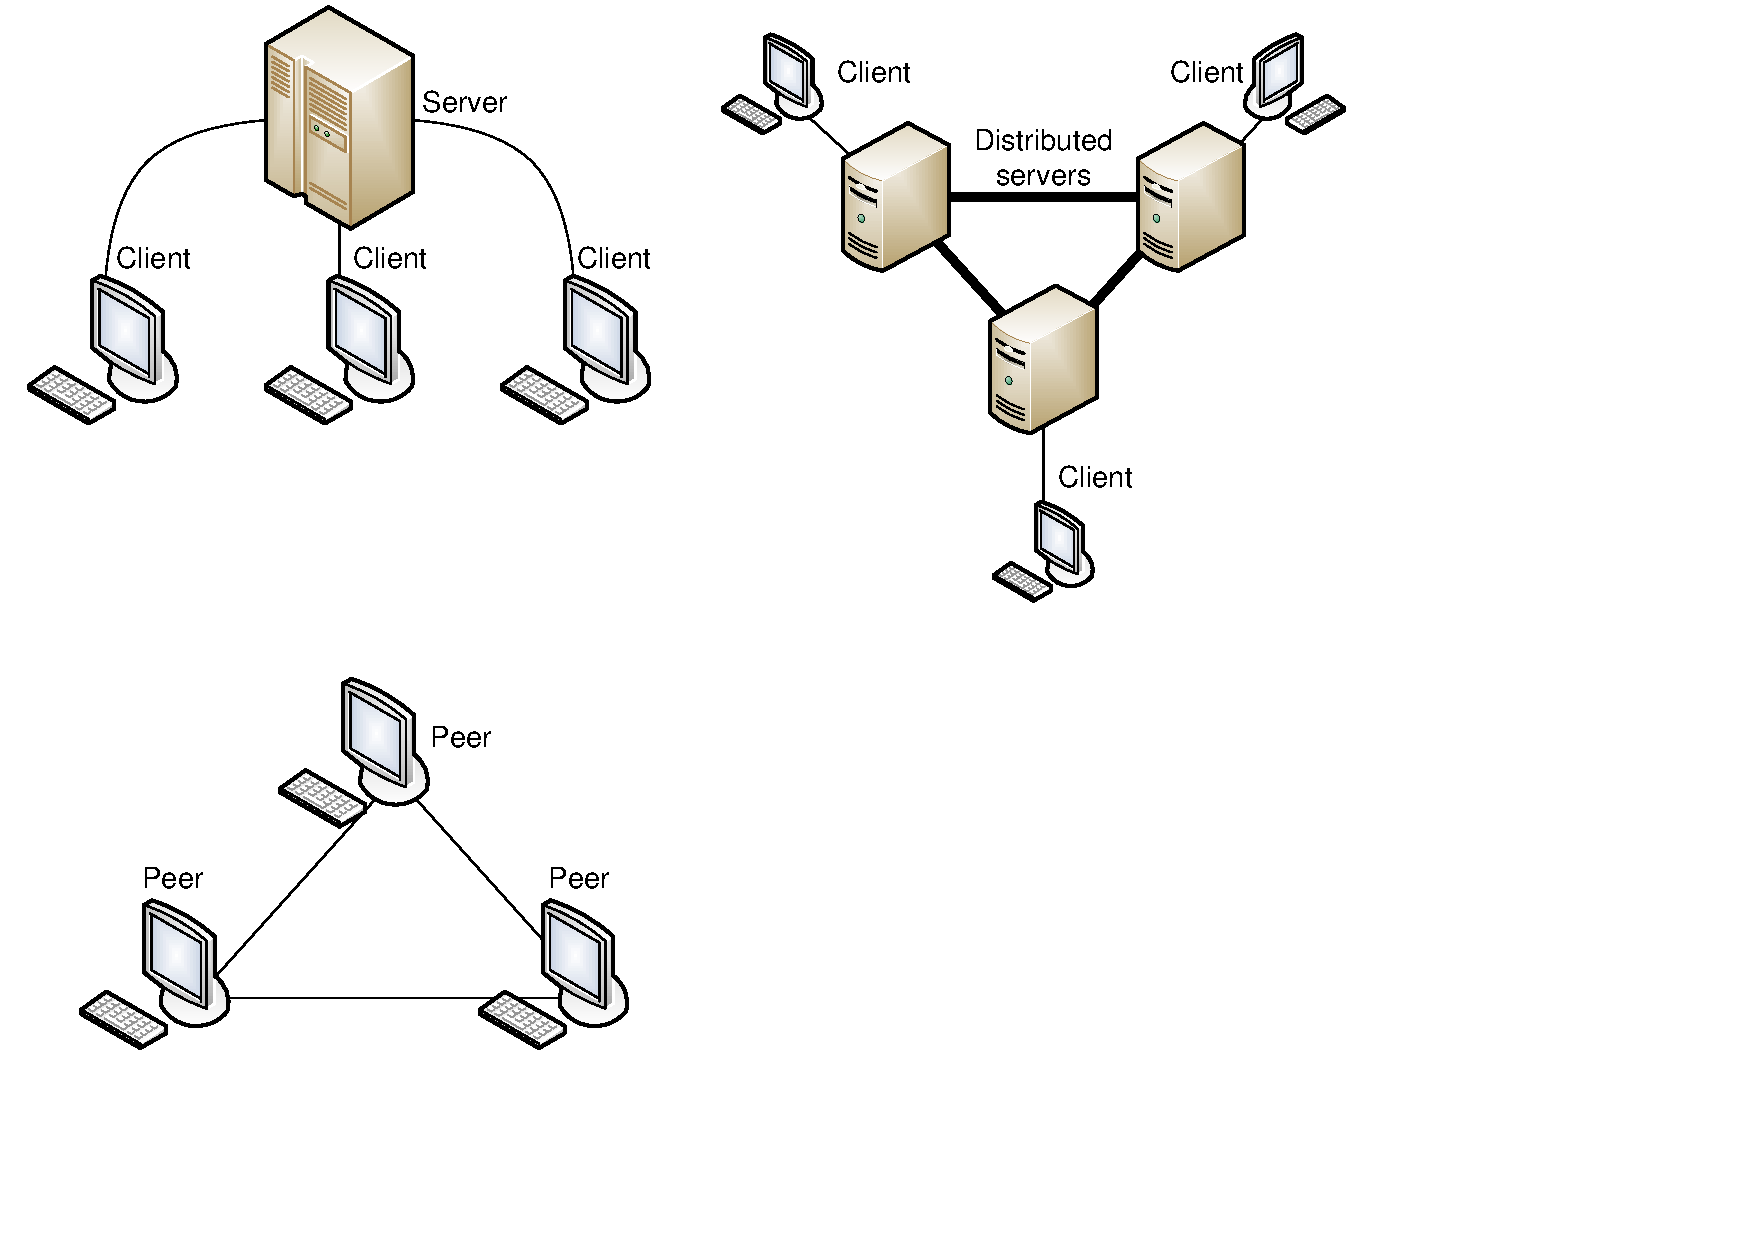
\includegraphics[clip=true, viewport= 0cm 12cm 11.5cm 21.5cm, width=0.5\columnwidth]{network_archs}}
\subfloat[Client/Multi-Server]{\label{fig_cms_arch}
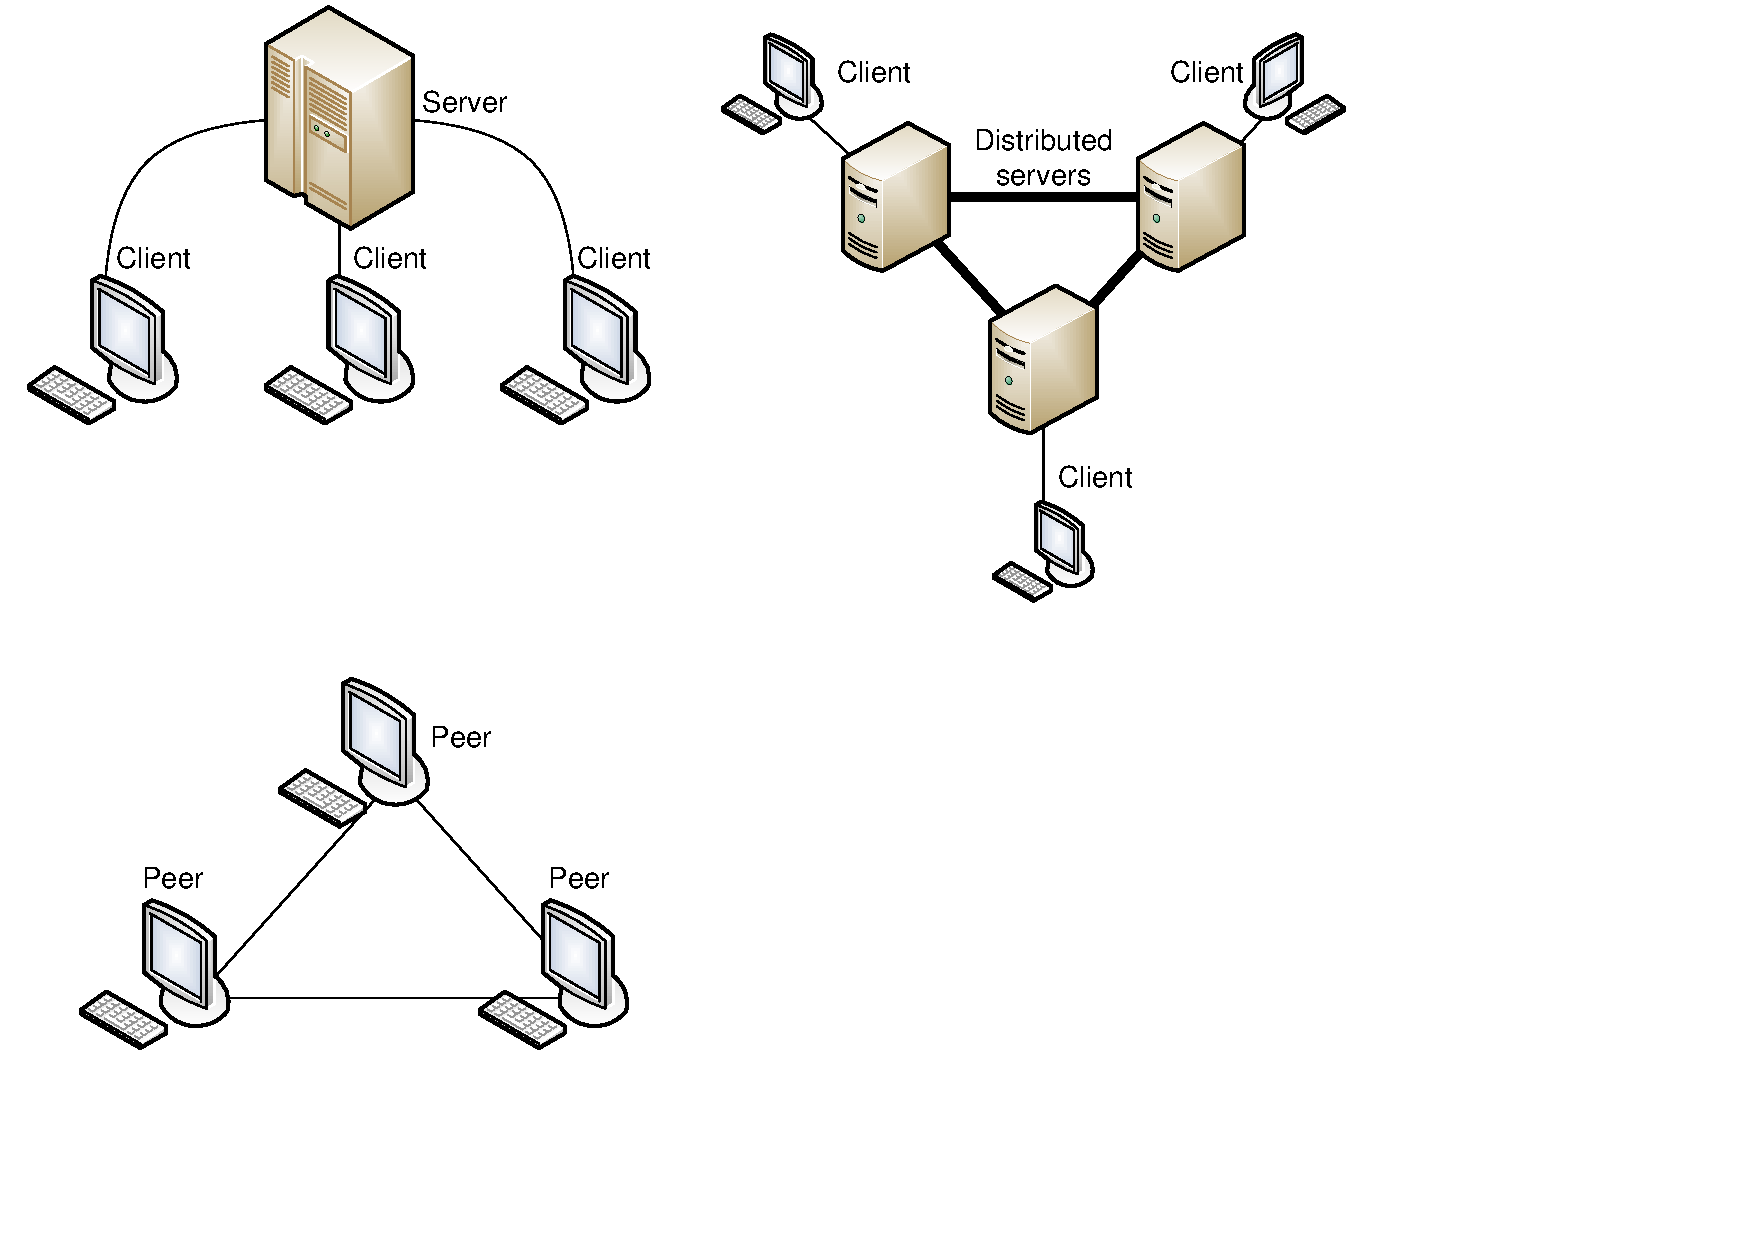
\includegraphics[clip=true, viewport= 12cm 10.5cm 23cm 21cm, width=0.5\columnwidth]{network_archs}}
\caption{Network architectures}
\end{figure}

Figure \ref{fig_cs_arch} shows the C/S model. The server is the entity on which the MMOG is hosted and is controlled by the game operator. The server contains the authoritative environment state, to which clients must revert if their states deviate from the authoritative state. Clients are computers operated by players, that connect to the server to play the game. The server is responsible for handling all queries from clients. Clients never communicate with other clients; they send their actions to the server and receive the updated states of other players from the server. All client environment states are non-authoritative.

\subsubsection{Advantages}

The C/S architecture has two main advantages that has made it the architecture of choice for all MMOG developers. Because of the centralised approach of the architecture, both administration and security are greatly simplified. Administration is simplified, because the game operator has full control over the server, server data and code. Efficient logging is also supported, because the server is able to not only log all server actions, but also all client actions.

Security is a significant issue in MMOGs, since some players sell in-game currency for real-world currency \cite{chinese_gold_farmer}. This makes the MMOG a platform that is capable of producing income, which increases the incentive of players to gain an unfair advantage over others. The more popular an MMOG, the greater the security threat. Because the operator has full control over the server code and is never required to furnish the
client with the server code, a potential attacker never has any knowledge of the server architecture and code. Because clients are never allowed to communicate directly, all malicious users can be filtered out of the network by the server when detected and even banned from the network.

Operators are able to ban players, since these games usually require a game account, which is linked to a copy of the game as well as some payment method. This introduces a large cost to players whose accounts are banned. The server or cluster is also housed in a secured location, where access can be controlled. These factors simplify the security of the C/S model by allowing the developers to place all intelligence in the server.

\subsubsection{Disadvantageous}
\label{classic_cs_disadvantages}

The C/S architecture has the following disadvantages: weak robustness, weak scalability, high cost to the operator, high latency, high amount of required server bandwidth and weak handling of transient loads.
\begin{itemize}
\item The robustness of the system is weak because it is a single point of failure. If the server fails or goes down for maintenance, the game is off-line and players are unable to play.

\item The system is also weakly scalable, since a single server cannot easily be extended with more resources. Even if an off-line approach is used, where hardware is upgraded after the system is taken down for maintenance, the hardware required to support a game hosting more than 3000 players, become prohibitively expensive, as described in Section \ref{mmog_cost}.

The server hardware should be able to support peak system loads, which means that sufficient resources should always be provisioned to support these peak load. This is not an economically viable solution, because resources to handle peak loads are not used most of the time. This translates to operators paying for the provisioning of resources, without having active players that pay for these resources.

\item Because no clients are allowed to communicate with other clients, every change that is made to the game world by a client, first had to be communicated to the server, which in turns relays this message to all clients after applying game logic and artificial intelligence (AI) algorithms. This two hop path, with the additional time for computation added by the server as well as possible buffering at the server when many clients communicate, significantly increases the latency of the system compared to a system where direct communication is used.
\end{itemize}

\subsubsection{Client/Multi-Server}

In an effort to address some of the C/S issues, the distributed C/S, also called the Client/Multi-Server (C/MS) model, was introduced, shown in Figure \ref{fig_cms_arch}. In a C/MS model,
the server functions are distributed amongst multiple machines to distribute the server load.

In general, the issues addressed and improved by the C/MS architecture are robustness, scalability, and peak load handling. The system is more robust, because the failure of one server will not necessarily lead to the failure of the whole system for certain system designs. The system is more scalable, because many less powerful servers may be used, which allows for the hosting of more players than what is currently possible with single server hardware. It also handles transient loads better, because, for cases where loads can be predicted, resources can by moved between servers to improve the user experience.

The disadvantages of this system is that the administration complexity is greatly increased. Such systems, although capable of handling many more users than a single server, is also more expensive. These disadvantages are, however, not technical problems and so it is assumed for current games, that these systems are what is required if a game is to be hosted for a large number of players.

\subsection{The cost of doing business}
\label{mmog_cost}

With the fast growing MMOG market, many companies are spending a significant amount of money to produce premium MMOG titles. Some development cost estimates are: \$18 mil. for Aion, \$20 mil., for Everquest \cite{aion_everquest_cost}, \$63 mil. for World of Warcraft \cite{wow_cost} and \$100 mil. to \$200 mil. for Star Wars: The Old Republic \cite{star_wars_cost_1}, \cite{star_wars_cost_2}. Although these figures are purely estimates, it does show that to develop a premium MMOG title costs a lot of money.

The issue with MMOG development is that, although they cost more to develop than single player or smaller scale multiplayer games, they are just as likely to fail. Despite this, game publishers are spending a lot of money in an attempt to recreate the success that is World of Warcraft.

Because of the large revenues being generated from MMOGs, many competitors are entering the MMOG space. Currently, the rate at which new MMOGs are added to the market is outstripping the growth of the market itself \cite{newzoo_mmo_report}. Furthermore, because of the recession, over the past two or three years, game subscriptions have been shown to stabilise or even decline \cite{mmo_growth_chart}.

The significant initial investment required to develop an MMOG also doesn't present the complete picture. Another factor driving up costs for an MMOG is the money required for server hardware, maintenance and support. An MMOG is not finished when it goes live. A team of developers is required to maintain the game, release patches fixing bugs and to produce more content to keep the player base sufficiently interested to ensure that players will continue to pay \$15 per month to play. Development and maintenance costs for World of Warcraft for four years is estimated at \$100 mil. to \$200 mil. \cite{wow_cost}.

With the costs involved, it is therefore difficult for a new developer to enter into this space. After the large initial investment into the game's development, all server hardware must be acquired and staff appointed to maintain the game. This money is spent before it is known whether the game will succeed or fail. It has been estimated that during the lifetime of an MMOG, 80\% of the game revenue goes into hardware and maintenance costs \cite{cs_mmog_cost}.

\subsection{The peer-to-peer proposal}

To our knowledge, the first distributed multi-user virtual environment was MiMaze, developed in 1998 by Gautier and Diot \cite{mimaze}. This revealed a new research field, which attempted to establish the peer-to-peer (P2P) model as a viable alternative to the classic C/S and C/MS architectures. In 2004, Knutsson et al. proposed the first scalable architecture to host massively multiuser virtual environments  \cite{knutsson_p2p_first}.

P2P MMVEs form the focus of this work. There are various advantages to moving from C/S to P2P in MMVEs. These include: increased robustness, improved scalability, lower operator costs, improved handling of transient player load and lower latencies. The advantages are described in Section \ref{p2p_mmve_advantages} in detail, but firstly it would be beneficial to acquire a greater understanding of the basics of the P2P network model.

\section{Peer-to-Peer networks}

A P2P network is a distributed network that exists out of many participating peers to fulfil some objective. In this work, a P2P network is defined as being a distributed network with the following properties
\cite{Rodrigues_acm_comms_p2p}:
%
\begin{itemize}
\item \emph{High degree of decentralisation}:  No or little centralised control exists. Server functionality is distributed amongst all peers.
\item \emph{Self-organisation}: Little or no self-organisation is required in the network. Peers are given an initial IP to allow them to join the network, but thereafter new neighbours are automatically acquired and peers remain connected to the network, even with other peers joining and leaving.
\item \emph{Multiple administrative domains}: Peers are not under the control of any single authority. Peers in the network belong to different organisations or individuals and direct administration is impossible.
\end{itemize}

P2P systems have been popularised by mainly three systems developed in 1999: the Napster music sharing service, the Freenet data store and the SETI@home volunteer-based distributed computing project. These three projects highlighted the advantages of P2P networks being: low barrier to entry, scalability, resistance to faults and attacks, and an abundance and availability of resources.

\subsection{The OSI model and P2P overlays}

\begin{figure}[htbp]
 \centering
 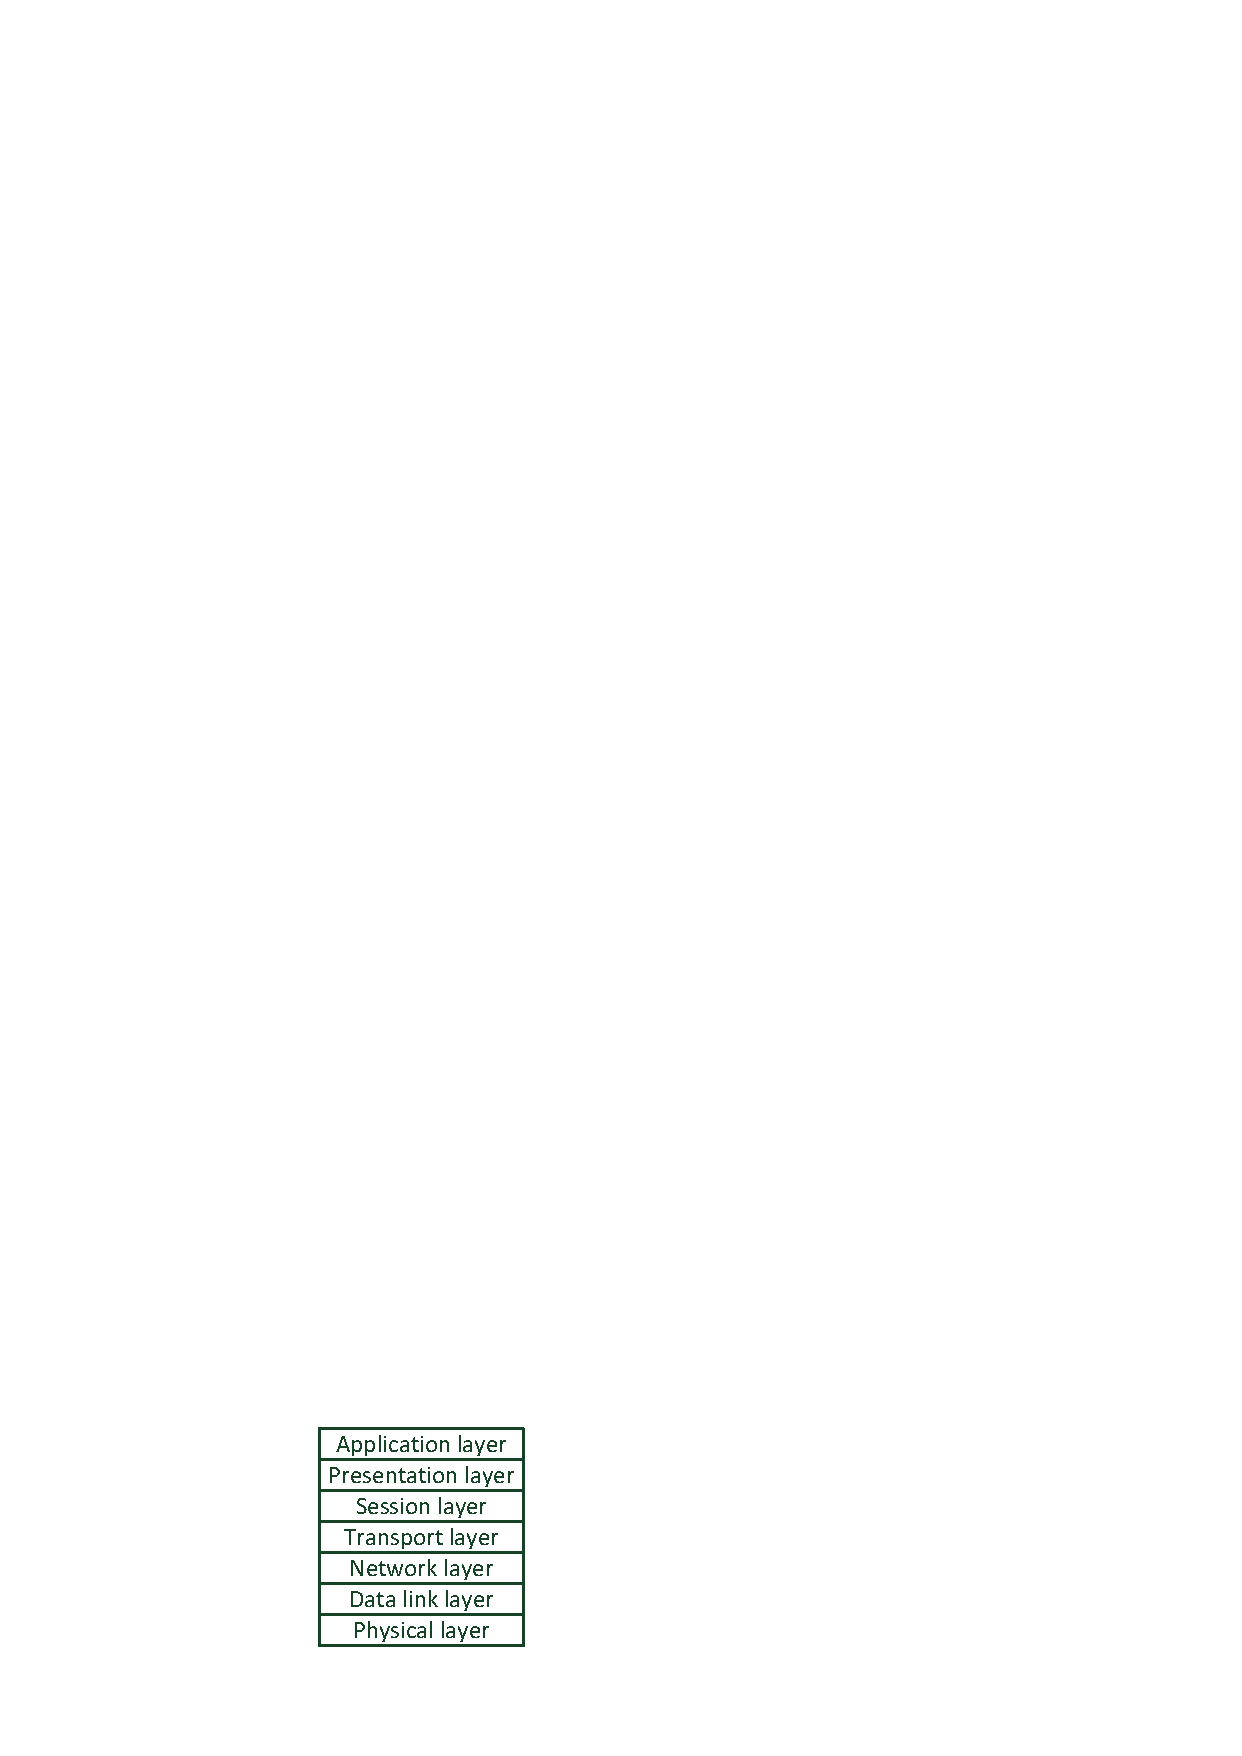
\includegraphics[clip=true, viewport=52.5mm 17mm 90mmm 56mm, width=0.4\textwidth]{osi_model}
 \caption{Layers of the OSI model}
 \label{fig_osi_model}
\end{figure}
%
A basis of computer networking is the layered architecture model, called the open systems interconnection (OSI) model \cite{OSI_protocol_stack}. It defines various protocol layers that allow for abstraction of complex operation in the lower layers in the higher layers. As shown in Figure \ref{fig_osi_model}, the OSI layers are, from bottom to top: the physical layer, the data link layer, the network layer, the transport layer, the session layer, the presentation layer and the application layer. In practice, the session, presentation and applications layers are usually all folded into the application layer.

The physical layer is the physical transmission medium and carries physical signals. Physical level protocol standards include: IEEE 802.11 (Wi-fi), USB, Bluetooth, etc.. The data link layer, sometimes referred to as the MAC layer in the Internet protocol stack, carries frames and is responsible for point-to-point data transfer on the same local area network (LAN). Signals from the bottom layer are converted into bits and sequences of bits are grouped into frames, which is seen to be sent over the data link layer. As can be seen, every higher layer abstracts elements of the lower layer to reduce complexity.

The network layer allows communication between different LANs, using routers, gateways and host addressing. Every computer in a network is referred to as a host. A well known network layer protocol is the Internet protocol (IP), which routes all Internet traffic. The transport layer is referred to as the end-to-end layer and represents the abstract connection between a source and destination host, where all intermediate routers and LANs may be ignored, since they are abstracted away by the network layer. Well known protocols in this layer include the user datagram protocol (UDP) and transport control (TCP) protocol. Above the transport layer, for the purposes of this work, is the application layer. The application layer has access to all network services, including routing and reliable transmission.

In the C/S architecture, the client and server are both located in the application layer and communicate with each other using the transport layer. They need not be aware of any of the lower layers.

P2P networks are created and maintained in the application layer of the OSI model, called the P2P overlay. An overlay is required so peers may know which other peers are part of the P2P network, since most nodes on the Internet will not be part of the network. The overlay is then defined by the routing table information stored on each peer. The overlay can be thought of as an additional layer in the OSI model. The overlay interfaces with the transport layer and P2P applications are one layer higher and communicate by using the overlay.

Peers in an overlay network might have neighbours that have no relationship to their physical position in the underlying physical network.

\subsection{Structured and unstructured P2P overlays}
\label{overlays}

Overlays can broadly be classified into structured and unstructured types. The classification is mostly based on the differing methods of routing and content retrieval in the network. This section only provides a brief comparison between structured and unstructured overlays. For a detailed comparison between the two types that also deals with many of the myths of structured overlays, please refer to \cite{Castro_structured_overlay_myths}.

With unstructured approaches, one is never assured that a data item will be retrieved, even if that data item is present in the network. If many duplicates of a data item are contained in the network, this becomes less of a problem, since it is assumed that the request will be routed to some set of peers that do  possess the item.

An unstructured architecture is well suited to content sharing and Voice over Internet Protocol (VoIP) networks, for example: P2P TV, BitTorrent, Gnutella and Skype. The reason for this is the high level of duplication in these networks, especially for popular content. It is also easier to perform keyword searches in unstructured networks and the overlay requires less maintenance.

Structured overlays have been proposed that provide for efficient routing and reliable retrieval of data items. Some well known structured overlays are: CAN \cite{CAN}, Chord \cite{chord}, Tapestry \cite{tapestry}, Pastry \cite{pastry} and Kademlia \cite{Kademlia_Maymounkov}. The basic principle of a structured overlay is that all nodes are identified by unique identifiers (IDs).

A popular method to create the IDs is to use hashes to a circular key space, using for example, the SHA-1 hash function. Any node in the overlay network is then able to efficiently route a query with a given ID, to a node with an ID closest to the given ID. An accurate comparison is that unstructured overlays are good at finding ``hay'', while structured overlays are good at finding ``needles'' \cite{Rodrigues_acm_comms_p2p}.

\subsection{Features of structured P2P overlays}
\label{structured_overlay_features}

A structured P2P overlay has certain key features that determines its lookup speed, space consumption and bandwidth requirement \cite{p2p_networking_handbook}. These features are geometries, routing algorithms, join/leave mechanisms, routing table maintenance and bootstrapping.

\subsubsection{Geometries}

An overlay's geometry determines how nodes are structured in the application layer network. The geometry allows for deterministic routing. The geometry determines the number of required lookup hops and how the network will be maintained during times when nodes join and leave the network, called churn.

\subsubsection{Routing algorithms}

The routing algorithm is directly related to the specific overlay geometry. The routing algorithm determines which nodes are traversed when a message is sent to a target node. The routing algorithm and the geometry determines the number of expected hops for a message to reach a destination.

\subsubsection{Join mechanism}

P2P networks experience constant churn, where nodes are joining and leaving the network. Mechanisms for a node to join the network should be present. This is usually in the form of a well known directory (bootstrap) server. When a node wishes to join the network, the directory server sends a set of nodes that the node may want to join.

\subsubsection{Leave mechanism}

If a node leaves the overlay, its neighbours have to be informed so they may update their routing tables. This is termed \emph{routing table maintenance} and has to happen every time a peer leaves the network. Neighbouring nodes of a node that left the network might also have to inform their neighbours of the change. Two types of routing table maintenance exist: opportunistic and active maintenance.

Opportunistic maintenance attaches routing information to existing request packets. Routing data is essentially ``piggy backed'' onto existing messages. This reduced messages overhead but the rate of routing table maintenance is directly proportional to the message rate. Active maintenance makes use of explicit update messages, which required more bandwidth but is more reliable.


\subsubsection{Bootstrapping}

After having been informed of a peer to join, a joining peer may initiate the process of positioning itself in the P2P network, called bootstrapping. This is the process of finding out where the joining node fits into the overlay in terms of the geometry. If the overlay requires that all nodes be connected in a ring organised by ID, then the joining peer must discover the nodes whose IDs are one more and one less than its own and join those two peers.

The process of bootstrapping is complete when a joining peer becomes a functioning member of the P2P overlay.

%TODO: Add something about the effect of the hashing and why it's important

\subsection{Advantages}

\begin{itemize}
\item P2P networks have a low barrier to entry, since little or no centralised infrastructure is required to maintain the system. This makes P2P networks inexpensive to operate and is one of the reasons Napster was able to provide its service for free.

\item P2P networks are considered scalable. Pure P2P networks can theoretically grow from hundreds to millions of peers, with the service remaining functional. This is all possible without the need for the operator to acquire more infrastructure, as opposed to the centralised client/server network, which required more powerful server clusters are the network grows to handle the growing number of client requests.

\item A P2P network is also resistant to faults and attacks, since the failure of a single peer has little to no effect on the network. This is because there are usually few peers that are critical to the correct functionality of the system. To incapacitate a P2P network, an attacker usually has to shut down a large proportion of the network.
\end{itemize}


\section{Peer-to-Peer MMVE network architectures}
\label{p2p_network_architectures}

P2P MMOGs are considered a sub-class of P2P Massively Multi-user Virtual Environments (MMVEs), a class that also includes large scale military simulators.

This architecture does, however, still have a few major issues that need to be solved before MMVEs can be developed that make use it. If these issues, discussed in Section \ref{key_challenges}, can be solved, a P2P architecture holds some powerful advantages over a C/S system.

The core idea of the P2P model is that each peer contributes sufficient resources to the network to host itself. This also means that all functions of the server in the classic C/S model are distributed amongst all peers. The authoritative environment state should now also be distributed amongst the peers in the network. Each peer will, therefore, contain a section of non-authoritative state for its own display purposes, and contain sections of the authoritative environment state.

\subsection{Advantages}
\label{p2p_mmve_advantages}

\begin{itemize}
\item The P2P architecture is robust, because there is no server that can fail, only individual peers. Individual peers failing will not affect any other peers other than the peer that failed. This behaviour makes game down-time extremely unlikely.

\item In P2P MMVEs, it is generally assumed that peers provide abundant and highly available resources, such as computation power, and long term and short term storage. Peers are usually personal computers, with gigahertz of processing power, multiple processing cores, gigabytes of short-term storage and terabytes of long-term storage space. In other words, it is assumed that P2P MMVEs do not consist of resource-constrained peers.

\item The system is scalable, because every peer essentially hosts itself.

\item Because of the high scalability, no extra resources are required from an operator perspective, when more peers join the network.

\item P2P networks also efficiently handle transient loads, since the joining peers contribute their own resources. If many players suddenly enter the
game no resource provisioning issues will arise, since peers already possess the required resources.

\item P2P architectures create a lot of opportunities for independent developers, because a large initial investment is no longer required to purchase
the expensive server hardware. Not only are hardware costs reduced, but running costs are also reduced.

\item Bandwidth required by the game server is now shared amongst users, which means that very little bandwidth costs will be incurred by the provider.

\item Latency is improved, because it is now possible to directly communicate between peers and it is not necessary to communicate via a server.
The distribution of the load as well as direct communication will further reduce latency.
\end{itemize}

\subsection{Requirements}

Key requirements have been identified for the creation of a P2P MMVE. What follows is an expansion and reinterpretation of the requirements identified by Schiele et al. \cite{Schiele_p2p_requirements}. Some of those key requirements, that are specific to P2P MMVEs, are briefly highlighted in this section.

\subsubsection{Distributed computation}
\label{distributed_computation_requirement}

Non-Player Characters (NPCs) are characters that are not controlled by any human player, but are rather controlled by some artificial intelligence routine or script executing on some host machine. These characters represent the traders and monsters in MMVEs and usually contain sets of rules that determine how they should interact with Player Characters (PCs) as well as their own state information. An NPC's state can be how much money and items it has to trade or how much health it still has after being attacked by a player.

Some game objects require computational power to function. An example of this is the Artificial Intelligence routines of NPCs or the computation of physics effects on in-game objects. In P2P MMVE, it might be required to distribute these computational tasks to offload computation load from peers that do not have sufficient resources.

\subsubsection{Consistency}
A key challenge with any networked game is how to maintain state consistency between users in the virtual world. In other words, to ensure that all users perceive a virtual world in the same state. Solving the state consistency problem for P2P MMVEs is one of the major development challenges and forms the focus of this work. The challenge of state consistency will be described in detail in Chapter \ref{chp:CONSISTENCY}.

\subsubsection{Persistency and state management}

P2P MMVEs require persistent state, which means that the information of users in the virtual world should be maintained. The items that a user possesses in the virtual world should remain on his virtual avatar, even if she logs out and later back on to the virtual environment.

Persistency is different to state management. Persistency is the long term storage of data, usually on secondary storage. State management deals with managing the state of objects in the virtual world. This includes handling all requests for that object from peers who do not yet possess the object, or processing changes that players have made to the objects in the virtual world.

\subsubsection{Interactivity}

P2P MMVE should be interactive and responsive. This means that they should support low latency interactions and possibly mask high latency operations, using techniques such as dead reckoning \cite{cheat_proof_playout}, so as not to break immersion. Interactivity means that all players actions should be handled as soon as possible.

\subsubsection{Scalability}

MMVE are by definition massive, supporting thousands to tens of thousands of players in the same virtual environment, as discussed in Section \ref{scalability_req}. A P2P MMVE should support as many users as a classic MMVE, preferably more.

\subsubsection{Security}

Security, which includes cheating mitigation, has been identified as a major issue for P2P networks \cite{knutsson_p2p_first}, \cite{challenges_p2p_gaming}, \cite{cheat_proof_event_ordering}. The challenges reside in the fact that peers are not under the control of the game producer. Since the authoritative environment state is distributed amongst peers, all peers have access to sections of the authoritative environment state. Peers also have access to the code that was classically only housed on the server. This creates the opportunity that peer might attempt to alter the authoritative state in ways that are not consistency with the environment rules.

One advantage that can be exploited to prevent cheating is that no peer contains all authoritative environment state and no single peer has more authority than another.

\subsubsection{Efficiency}

The network architecture of a P2P MMVE should be efficient. This usually goes without saying, but the reason why it is specifically stated is because the P2P network architecture basically implements the functionality of the server in the classic server model.

The server functionality has to be distributed accross all users of the P2P system. In addition to server functionality, a peer still requires the functionality of a classic client as well. This means the rendering of intricate graphics and calculation of complex physics. The P2P MMVE network architecture should, therefore, require as little as possible resources, of the resource that would ordinarily have been used for graphics and physics.

\subsubsection{Incentives}

P2P schemes require all players to share resources in order to ensure correct functionality. Players might, however, not want to share their resources, whilst still benefiting from the resources of others. The purpose of incentive mechanisms is to ensure that all players contribute resources, by incentivised contribution.

All distributed resource sharing models require incentive mechanisms. For example, Bittorrent systems use the tit-for-tat protocol to ensure that all people downloading data are also contributing data \cite{tit_for_tat}. Such mechanisms are also required with P2P MMVEs. One advantage in designing an incentive mechanism for a P2P MMVE is that players can be made to contribute resources for the duration of play. The issues with file sharing systems are not present where a peer, after downloading a file, has no more incentive to contribute.

\subsection{Key challenges}
\label{key_challenges}

Using P2P MMVEs has many advantages, but some challenges still remain. The main challenges are state consistency, limited peer bandwidth, cheating mitigation, incentive mechanisms and distributed computation. This section will present some information on work that has been done in the different areas and talk about the maturity of the various solutions. In general though, most solutions are still research projects and none have yet been implemented as commercial products.

\subsubsection{Peer bandwidth}
\label{peer_bandwidth_usage}

In a paper by Miller and Crowcroft, a packet simulator was created to determine the required bandwidth and effective latency, if a game such as World of Warcraft were to be implemented using P2P technologies \cite{Miller_p2p_infeasability}. Their simulation results indicate that today's networks are not able to host P2P MMVEs, with the required bandwidth and latency constraints. Such a significant result requires verification, but at the least, it shows that reducing bandwidth and latencies for P2P MMVEs should be a primary design requirement.

\subsubsection{Cheating mitigation}
\label{key_challenges_cheating}

There are various security issues that are usually classified according to the level in the OSI protocol stack where they occur. The areas identified by \cite{cheat_proof_event_ordering} and expanded upon by \cite{cheating_taxonomy} are: game level, application level, protocol level and infrastructure level. The description is consistent with the generally used layered security model \cite{distributed_systems_security}.

\begin{itemize}
\item Game level cheats are ways in which a malicious player may gain an unfair advantage over other players, within the confines of the game. These cheats are usually because of software bugs and some examples are duplication and teleport cheats.

\item Application level cheats are where malicious players alter the game software to gain an unfair advantage. This is usually done by gaining access to the game state to which they should not have access at the current time. An example of this is ``map reveal'' cheats in strategy games, where the ``fog of war'' is removed and the player can observe all the opponent's movements. Other cheats that are used include augmenting the player's UI with extra information that allows the player to make more informed decisions.

\item Protocol level cheats are cheats based on the different methods of communicating data across the system. These usually concern dropping, delaying of modifying IP packets to achieve certain outcomes in the game.

\item Infrastructure level cheats concern exploiting the underlying infrastructure on which a game is built. Types of infrastructure cheats include denial of service (DOS) attacks on the P2P overlay to prevent messages that should be forwarded by a peer from being forwarded.
\end{itemize}

As with all taxonomies, all cheats may not cleanly fit into one if these boxes, some cheats may occur over multiple levels or a cheat with a specific outcome can be implemented differently on different levels. The field of P2P security has recently received more attention than in the past and has started to bear fruit \cite{survey_p2p_game_cheats}.

This is, however, an ongoing research field with many issues still open. For an in-depth review of the security issues facing peer-to-peer system in general, refer to \cite{p2p_security_issues}. These issues are the same issues facing P2P MMVEs, with the exception of the game and application layer issues.

\subsubsection{Incentive mechanisms}

Some proposed incentive schemes increase a player's reputation when resources are provided  \cite{classic_p2p_reputation} \cite{proactive_reputation}. This might create a type of meta game, where players try to gain as much reputation as possible. It can however be argued that this scheme does not really enforce the provisioning of resources. A player who does not want to provide resources might not see a higher reputation as sufficient incentive to provide resources.

Other issues with incentive schemes is that sometimes players might have insufficient resources. Such players should be aided by other players with sufficient resources and not be disallowed from playing the game. When limited resources are taken into account, the issue of reporting a false amount of available resources becomes a problem. A peer that has sufficient resources, might report insufficient resources, to avoid being penalised. It is evident that there is a need for more research in this field.

\subsubsection{Distributed computation}
\label{distributed_computing_challenge}

Some architectures assume that the computational requirements will be fulfilled where the object state is hosted \cite{solipsis}, but other schemes exist that allow for the CPU power to be distributed amongst peers. One such scheme makes use of a ``job board'' like mechanism, where tasks are advertised on specialised peers. All peers monitor these specialised peers and may elect to perform the advertised tasks \cite{fan_mediator_paper}.

\subsubsection{State consistency}

The state of the art of state consistency techniques will be reviewed in detail in Chapters \ref{chp:CONSISTENCY} and \ref{p2p_MMVE_state_persistency}.

\section{Research objectives}

The objective of this work is to design and develop a novel state management and persistency architecture, specifically designed for P2P MMVEs, that satisfies all P2P MMVE storage requirements and takes into account the requirements of the consistency architecture in which it will operate.

\section{Related work}

The basis for this dissertation is the work done by Lu Fan, in his dissertation entitled: ``Solving Key Design Issues for Massively Multiplayer Online Games on Peer-to-Peer Architectures'' \cite{Fan_phd} as well as the paper by Fan et al.: ``Design Issues for Peer-to-Peer Massively Multiplayer Online Games'' \cite{Fan_deisgn_issues_p2p}.

In the works by Fan, a survey is performed as to the main challenges that are still present with P2P MMVEs at that time (2009). The main challenges are identified as interest management, event dissemination, cheating mitigation, task sharing, incentive mechanisms and state persistency.

Fan states that: ``Game state persistency is a major challenge for P2P MMVEs as existing P2P storage infrastructures are designed to support file sharing, and seldom fulfil the performance and security requirements of a MMVE. \ldots the persistency area is still immature with many problems waiting to be investigated.'' \cite{Fan_phd}.

Fan, however, does not focus on solving state persistency issues of P2P MMVEs. A focus is instead placed on self-organisation in the P2P network, super peer selection, fault tolerance mechanisms, membership management mechanisms, heterogenous task mapping and an accounting scheme for interest management \cite{Fan_phd}. The Mediator framework is designed and the novelty is reported to be the task mapping infrastructure that allows processing jobs to be advertised on a job-board system for other peers to perform, thereby sharing the processor load of all peers in the network \cite{fan_mediator_paper}. A brief overview of this work is presented in Section \ref{distributed_computing_challenge}.

Recent work that is most similar to ours is the dissertation by Varvello entitled: ``A Peer-to-Peer Architecture for Networked Virtual Environments'' \cite{varvello_phd}. They develop P2P Second Life by altering the Second Life implementation to run over an existing P2P file sharing network, called KAD \cite{KAD_Steiner}, which runs on the Kademlia P2P routing overlay \cite{Kademlia_Maymounkov}. Their focus is thus on a practical implementation, taking an already implemented MMVE and running that as a P2P system over an already implemented P2P network. They also design and simulate a responsive distributed storage system for P2P MMVEs, called Walkad \cite{Walkad_Varvello}. Walkad is deployed to a cluster and ModelInet \cite{ModelInet_Vahdat} is used to emulate wide-area latencies in the cluster underlay. A synthetic Internet topology is generated to model the wide-area latencies, using Inet \cite{Inet_warwick_jamin}.

There are some similarities between Pithos and P2P Second Life. Both provide the design and implementation of a storage system for P2P MMVEs, although the designs are very different as will be explained shortly. Some of the requirements for P2P MMVE state management and persistency were also identified by P2P Second Life, these are: scalability, security and responsiveness. Additionally we identify reliability and fairness as key to designing the P2P MMVEs of the future. We argue for the various identified requirements from the perspective of the generic consistency model that we design. Both our systems also make a distinction between local and non-local storage requests, since it is recognised that users have a finite Area of Interest (AoI).

The KAD P2P network is, however, a file sharing network where user profiles, such as session time, do not necessarily model user lifetimes in P2P MMVEs. It is also not possible to control the parameters of the peers in the network, such as churn. The Walkad simulation is also on a relatively small scale, running on 1024 peers with less than 600 objects in the virtual environment.

Our design philosophy was to design a P2P storage architecture from the ground up, for the P2P MMVEs of the future, supporting thousands of peers and able to store hundreds of thousands of objects. In order to evaluate our design, we elected to implement it in the form of a large scale network simulation based on the Omnet++ network simulator. This allows for thousands of nodes and hundreds of thousands of objects to be simulated, with realistic latency characteristics in the underlying network based on real-world Internet measurements. In our simulation, most results are shown for a smaller network of 2500 nodes, but in order to show the scalability of our system we also simulate it for 10,000 nodes and millions of objects.

The design philosophy of our storage system compared to that by Varvello is also different. They use a cell-based storage system, where each cell has multiple coordinators. Each cell coordinator replicates all the objects of the cell it coordinates. Our storage system is a group based system, where users are dynamically grouped and objects are stored in groups, rather than cells. Our system also attempts to distribute the load to all peers in the group, by having all group peers store objects. In P2P Second Life, only cell coordinators store objects in the cell. Avatars in the cells do not store objects for that cell.

In terms of performance, there is also some difference between Pithos and P2P Second Life. The responsiveness of Walkad, the improved storage systems developed for P2P Second Life, varies from $O(1)$ in the best case, for local queries to $O(N_c)$, also for local queries, where $N_c$ is the number of cells in the virtual world. The actual performance depends on how equally all regions of the virtual environment are partitioned. If all environments are partitioned exactly the same number of times, requests to neighbouring cells have $O(1)$ responsiveness. Our storage system has a fixed performance of $O(1)$ for local (group) queries. For non-local queries, both our storage systems have order $O(\log (N))$ performance, but again using different implementations.

For our design, the bandwidth requirements of the different methods are also evaluated, since bandwidth usage of P2P systems is of great importance as discussed in Section \ref{peer_bandwidth_usage}. Bandwidth usage is not something that is evaluated in P2P Second Life.

Pithos is also evaluated from a security perspective. Some designs that improve security are presented and evaluated for various percentages of malicious users in the network. In the work on P2P Second Life, security is stated as being of high importance, but the system is not designed for security or evaluated in an environment containing malicious peers.

%=======================================
% Varvello
%=======================================
% Similarities
%=======================================
%Similar requiremens than what we observed:
%Recognises the need for responsiveness.
%Need for consistency
%Scalability
%Persistency (Reliability)
%Does not look at reliability per se, but measures how long objects remain alive. (Object lifetime measurements)
%Security is mentioned as important, but that it will not be addressed.
%Recognise difference between local and non-local queries

%=======================================
% Object management
%=======================================
%===============================================
% Main disadvantages, compared to Pithos design
%===============================================

%Does not address dynamic object creation and removal. In Pithos peers constantly generate objects and other peers have to be made aware of the new objects.

%Bandwidth usage is not discussed

%simulate for maximum of 586 objects, we do hundreds of thousands per group
%Limited number of nodes (max 1024), we simulate from 2500 to 10,000

%Dynamic regioning is performed during the initialisation phase, and never afterwards. It unsure how the system will be impacted with dynamic object creation.

%Naive approach has lower theoretical responsiveness. Walkad also has lower theoretical responsiveness.
%Little chance of cells being all on the same level, that would require equally spaced objects throughout the virtual world. Note: This is stronger than uniform spacing.

%Queries require a single routing hop per cell in the range query for direct neighbours and O(log(N)) outside.

%Does not deal with security (no quorum mechanisms)

%===============================================
% Other observations
%===============================================
%Local queries used to for state display (while walking and running)
%150ms latency for local queries
%200ms for non-local queries

%Does not evaluate underlying network architecture
%Look at reference 90 for KAD user session characteristics
%Kademlia also requires O(log(N)) routing time
%Also uses TTL of 24 hours

%State that their contribution isn't the design of the storage architecture, but rather how they adapted KAD to handle object storage and retrieval is (For the naive implementation).

%Use R cell coordinators, where R replicas of an object are stored on each of the R cell coordinators.
%So many peers are chosen as coordinators that all peers equally share the load i.t.o. cell IDs manageed.
%This is stated as the main method of load balancing.
%Nothing is stated about the actual amount of data shared.

%Their system showed 0.7 persistency during the time which objects were begin dynamically created.

%Walkad doesn't deal with avatars, because avatars move around constantly and that required constant updates to the objects. Avatars moving require constant repartitioning of the world (which would drastically decrease consistency).

%Walkad can be integrated into Pithos's overlay storage to further improve performance.

%Dynamic regioning

%No distinction is made between state management and state persistency

%Focus on consistency, while we focus on the authoratitive store itself.

%=======================================
% Questions
%=======================================
%How is a cell coordinator chosen? If there are between 10 and 20, how is one selected?
%Do coordinators experience churn?
%What are those 30\% statistics and why are they so low?
%What are KAD node lifetime statistics?
%When node balancing is tied to the management of cell-IDs, are active and control cells regarded as equal?

%=======================================
% Avatar management
%=======================================

\section{Contributions}
\label{objectives}

\begin{itemize}
\item A generic state consistency model is developed that encompasses both C/S and P2P consistency models. This is presented in Chapter \ref{chp:CONSISTENCY}.

\item A review of various state management and state persistency systems is performed in Chapter \ref{p2p_MMVE_state_persistency}.
    \begin{itemize}
    \item The state management survey identifies some key metrics by which state management systems may be compared, namely: fairness, reliability, responsiveness, scalability and security.
    \item Storage types described in the literature are found to be classifiable as super peer storage, overlay storage, hybrid region-based storage and distance-based storage.
    \item A journal survey paper has been published on this work, appearing in the IEEE Transactions on Parallel and Distributed Systems \cite{gilmore_p2p_mmog_state_persistency}.
    \end{itemize}

\item A novel state management and persistency architecture, called Pithos, is proposed and then implemented in simulation. Pithos increases reliability and responsiveness compared to classic P2P MMVE state persistency methods.
    \begin{itemize}
    \item Two types of storage implementations (safe and fast) are evaluated, with fast storage found to be more applicable to P2P MMVEs.
    \item Three types of retrieval (fast, parallel and safe) are evaluated and are all found to be useful in different situations.
    \item Two types of repair are evaluated (periodic and leaving), with leaving repair found to be more adaptable to changing network conditions.
    \item The design, implementation and initial evaluation of Pithos has been published at the International Workshop on Massively Multiuser Virtual Environments (MMVE) at the IEEE International Symposium on Audio-Visual Environments and Games (HAVE) \cite{Pithos_mmve_2011}.
    \end{itemize}

\item A statistical model, using a Markov chain, is developed to predict expected object lifetimes and is used to verify the Pithos results. The model can be used to design distributed storage systems for required mean object lifetimes.
\end{itemize}

\section{Summary of this work}

In order to design a state management and persistency architecture for P2P MMVEs, the environment in which such an architecture will function first has to be understood. This environment was found to be the consistency model of the P2P MMVE. In Chapter \ref{chp:CONSISTENCY}, a study is undertaken to determine all the required parts of a consistency model. From studying the literature on classic consistency architectures, as well as the literature on modern P2P MMVE consistency architectures, a generic consistency architecture was developed. Both P2P MMVE state consistency or C/S state consistency are all specialised cases of the generic model.

All modules that form part of the generic consistency model are described, and a summary of research into the various fields are presented. During the investigation of the consistency model, state management and state persistency are found to form part of state consistency in the authoritative storage module.

Knowing that state management and state persistency will be required by the consistency model, the other modules that interface with the authoritative storage module are investigated. These are found to be the environment logic module and object update module.

Chapter \ref{p2p_MMVE_state_persistency} explores the various state management and persistency schemes described in the literature. It first defines key requirements that state management and persistency architectures should possess, based on what was learned in Chapter \ref{chp:CONSISTENCY}. Key requirements are found to be: fairness, reliability, responsiveness, scalability and security. The storage types reviewed were found to be broadly characterisable into: super peer storage, overlay storage, hybrid region-based storage and distance-based storage. A discussion of each storage type is presented in terms of the requirements identified earlier.

It is found that none of the storage types currently available in the literature satisfy all the identified requirements. Chapter \ref{chp:DESIGN} presents the design of a novel state management and persistency architecture, called ``Pithos'', to satisfy all identified requirements. Pithos is designed as a hybrid storage, containing slower, but scalable overlay storage and faster but non-scalable group storage.

The design firstly describes which modules and mechanisms are used to satisfy the P2P MMVE state management and persistency requirements identified in Chapter \ref{p2p_MMVE_state_persistency}. Chapter \ref{chp:DESIGN} also presents the Pithos design from a use case perspective, showing how the other modules, identified in Chapter \ref{chp:CONSISTENCY}, are allowed to interact with Pithos. The design of each module and mechanism is described on a conceptual level, without referring to any specific implementation environment.

Chapter \ref{chp:IMPLEMENTATION} describes how Pithos is implemented in the simulation environment, called Oversim. The chapter first provides a motivation for selecting simulation and Oversim as the implementation environment. It also describes how Oversim is expanded to allow for the complete generic state consistency model developed in Chapter \ref{chp:CONSISTENCY} to be integrated into it. Pithos nodes are then described in terms of their Oversim module implementations. The chapter also presents some of the major implementation specific issues encountered during the implementation of Pithos, along with the chosen solutions. Specific attention is paid on how group consistency was ensured. The implementation of the application driving Pithos, called PithosTestApp, is also presented.

Chapter \ref{chp:EVALUATION} provides an evaluation of Pithos in terms of the requirements identified in Chapter \ref{p2p_MMVE_state_persistency}. Pithos is found to have high reliability, while having a responsiveness of 1.6 hops in the best case. Responsiveness is found to heavily depend on the underlying network architecture, as well as the probability of inter-group, compared to intra-group requests.

The bandwidth requirements of Pithos are also presented and found to be in the order of tens of kilo bits per second, but depending on the size of the object stored in the system. It is found that Pithos generates 88\% overhead, when compared to the data received and sent to the higher layer. Data is defined as only the data of a stored object, ignoring any packet header information received and sent from and to the higher layer and ignoring any responses not containing object data sent and received to and from the higher layer.

Of the overhead generated by Pithos, it is found that the group storage section of Pithos requires only 14\% overhead, but that the overlay storage section, which is based on a third-party implementation, requires 86\% overhead.

The fairness of Pithos is evaluated and found to compare well with that of overlay storage.

The Pithos implementation is evaluated for various percentages of malicious peers present in the network, that modify all objects requested from them. The quorum mechanism implemented in Pithos is shown to improve retrieval reliability for relatively large percentages of malicious nodes present in the network.

Finally, the results of the object repair mechanism, by which Pithos ensures long-term object survival is shown. It is found that object survival, which is of high importance when designing a distributed storage system, depends heavily on the repair rate, number of initial replicas and expected object lifetime.

Chapter \ref{chp:MODELLING} extends an existing statistical model, to improve the accuracy of object lifetime predictions in networks, such as Pithos, where group size is limited. This is done using an expanded Markov chain model, which allows for the theoretical predictions of object lifetimes. The theoretical predictions are verified using the Pithos implementations and found to closely match.

Chapter \ref{chp:CONC} summarises the main results found in this work. It also presents a discussion of future work that might be undertaken in each of the areas where this work provided contributions.
